\chapter{Project Design} 

\section{Overall Architecture}

\begin{figure}[H]
	\centering
	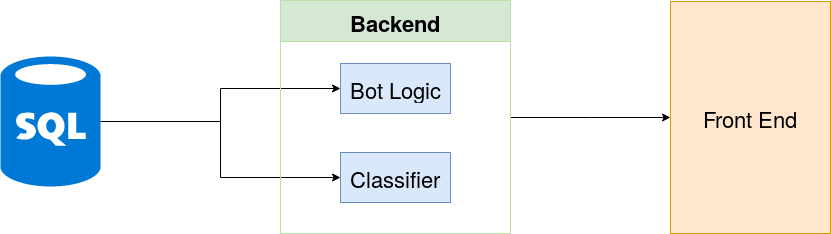
\includegraphics[width = \textwidth]{Architecture}
	\caption{Overall architecture}
	\label{archi}
\end{figure}

\section{Database}

\paragraph{}
We searched for a public database of symptoms and diseases but those database are not directly usable. So we created our own database with truth worthy data publicly accessible.
\paragraph{}
In the area of medicine and health care it is a well known fact that there is a lot of data and many different aspects that can be considered when taking a decision or making a diagnosis. 
\paragraph{}
After analyzing the data itself we decided that we will choose the relational data model (see figure \ref{db}).
The reason is that we have a lot of data that can be dependent upon other data.
\paragraph{}
One obvious and clear example is the disease’s dependency upon symptom(s).\\
\\
Example :
\paragraph{}
Someone has the following symptoms : high temperature, fever, cough, tiredness and sweating. \\
Obviously, assuming all of those symptoms we can conclude that the person might has flu. But if the person was complaining about low temperature instead of high temperature, we would most likely assume pneumonia as a state of the condition. The reason is that low temperature combined with the other symptoms is more typical for pneumonia than flu. \\
Both of the examples show how we can differ our decisions from one to another and how we make decision according to the chosen decision-making strategy. In other words diagnosis or more specifically final disease is the decision and the symptoms are defining our basic decision-making strategy.\\
\\
$High\ temperature, fever, cough, tiredness, sweating \rightarrow Flu$\\
$Low\ temperature, fever, cough, tiredness, sweating \rightarrow Pneumonia$\\
\\
$Basic\ decision\ making\ strategy : Symptoms$\\
$Decision : Diseases$\\
\\
There is an alternative interpretation that is valid for the upper case. 
We can say that we can invert the roles and we will still have true logic.\\  
So we will have this :\\
\\
$Flu \rightarrow High\ temperature, fever, cough, tiredness, sweating$\\
$Pneumonia \rightarrow Low\ temperature, fever, cough, tiredness, sweating$\\
\\
$Basic\ decision\ making\ strategy : Diseases$\\
$Decision : Symptoms$\\
\\
To summarize we can say that the data dependency is bidirectional.\\
\\
$Flu \leftrightarrow High\ temperature, fever, cough, tiredness, sweating$
\paragraph{}
This is leading to the biggest problem – data handling.
In other words  we are forced to use many-to-many relationship model which is leading to a difficulties in data inserting and Big Data.

\section{Database structure and design}
\paragraph{}

\begin{figure}[H]
	\centering
	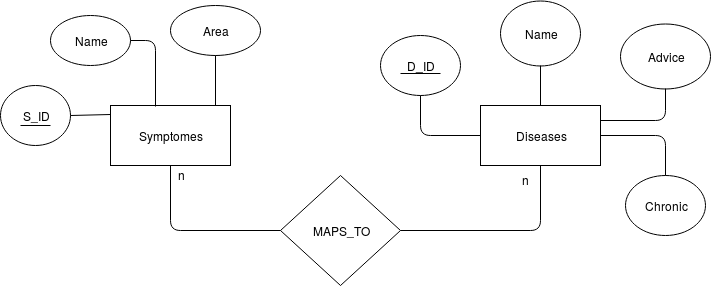
\includegraphics[width = \textwidth]{DB}
	\caption{Database design}
	\label{db}
\end{figure}

\begin{figure}[H]
	\centering
	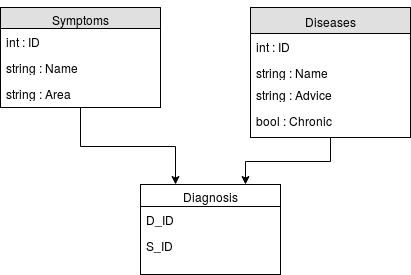
\includegraphics[width = 0.7\textwidth]{UML}
	\caption{Database structure}
	\label{uml}
\end{figure}

\section{Data model}
\paragraph{}
We have 3 tables in our relational database.
\paragraph{}
Symptoms – id, name and area which the symptom occurs. \\
Diseases – id, name, advice (medical advice if you are in that condition), chronic(boolean value used to show us if the disease is chronic or not)\\
Diagnosis – table connecting the symptoms with the diseases by ids.
\paragraph{}
A problem that occurs in our project is finding trustworthy data. The data we are using is taken from Mayoclinic\cite{bib:misc:4}.
\paragraph{}
The development team of the website consists of experts in the medical field. 
Physicians, scientists and other medical experts contribute to the website with their knowledge and experience. That’s the main reason why we decided to trust this website and use the data from it.   
\paragraph{}
As you can see on the figures \ref{uml} and \ref{db} it is complicated to insert data in the database.
With the current design and structure it’s impossible to join the tables symptoms and diseases because of the data dependency. As a result, while inserting data, every time we should fill the data in the diagnosis table to have the connection between every symptom and disease at the end. 
The other problem is that the more data we are inserting the bigger becomes the diagnosis table. That means that at some point we are going to face the big data problem.
\paragraph{}
For future development, solutions for cloud database might be considered but because of the big data either the design should be changed or some optimization techniques should be used on the data. Otherwise bottleneck may appear in a result of the growing data. 

